\begin{theo}[Magnetisch veld ten gevolge van een rechte draad]{Magnetisch veld ten gevolge van een rechte draad}
    \begin{minipage}{0.87\textwidth}
        Het magnetische veld ten gevolge van de elektrische stroom in een lange rechte draad is zodanig dat de
        veldlijnen cirkels zijn met de draad in het midden (zie figuur). De veld sterkte is groter hoe dichter je bij de
        draad bent en hoe groter de stroom, in formulevorm:
        \begin{equation*}
            B \propto \dfrac{I}{r}
        \end{equation*}
        met r de loodrechte afstand van de draad. Deze relatie blijft waar als we aanemen dat de draad lang is.
        Het magnetisch veld nabij een lange, rechte draad is als volgt
        \begin{equation*}
            B = \dfrac{\mu_0}{2\pi}\dfrac{I}{r}
        \end{equation*}
        met $\mu_0$ de magnetische permeabiliteit in vacuum.
    \end{minipage}
    \begin{minipage}{.09\textwidth}
        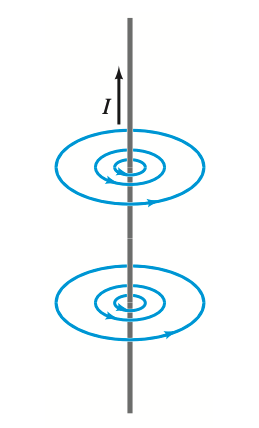
\includegraphics[scale=0.225]{Images/Magnetisme/MagnetischVeldTenGevolgeRechteDraad}
    \end{minipage}
\end{theo}

\begin{app}[Magnetische kracht tussen twee parallelle draden]{Magnetische kracht tussen twee parallelle draden}
    \begin{minipage}{0.77\textwidth}
        Neem twee lange evenwijdige draden gescheiden door een afstand d, zoals in de figuur. Ze voeren respectievelijk stromen $I_1$ en $I_2$.
        Elke stroom produceert een magnetisch veld dat door de ander wordt ‘gevoeld’, dus oefenen ze een kracht uit op mekander. We weten dat
        \begin{equation*}
            F_{\text{max}} = I\ell B
        \end{equation*}
        en dus krijgen we:
        \begin{equation*}
            F = I_{2}B_{1}\ell_{2} = \dfrac{\mu_0}{2\pi}\dfrac{I_{1}I_{2}}{d}\ell_{2}
        \end{equation*}
    \end{minipage}
    \begin{minipage}{.19\textwidth}
        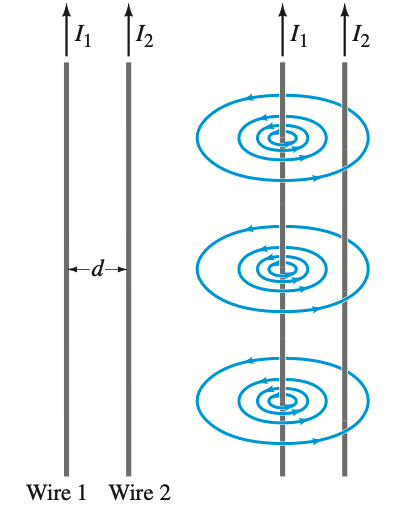
\includegraphics[scale=0.225]{Images/Magnetisme/MagnetischeKrachtTussenTweeParallelleDraden}
    \end{minipage} \vspace{0.2cm}\\
    Hieruit kunnen we afleiden dat evenwijdige stroomvoerende geleiders elkaar
    \begin{itemize}
        \item aantrekken indien de stroom in dezelfde richting vloeit,
        \item afstoten indien de stroom in tegengestelde richting vloeit.
    \end{itemize}
\end{app}

\begin{lem}[Ampère]{Ampère}
    De lijnintegraal van het magneetveld langs een gesloten pad is gelijk aan $\mu_{0}I_{\text{in}}$, waarbij $I_{\text{in}}$ de totale stroom is, die vloeit door een oppervlak dat omsloten is door het pad, in formulevorm:
    \begin{equation*}
        \oint \Vec{B} \cdot d\Vec{\ell} = \mu_{0}I_{\text{in}}
    \end{equation*}

\end{lem}